\documentclass[11pt]{article}
\usepackage[pdftex]{graphicx}
\usepackage{siunitx}
\usepackage{amsmath}
\usepackage{fixmath}
\usepackage[czech]{babel}
\usepackage[utf8]{inputenc}
\usepackage[T1]{fontenc}
\usepackage{enumitem}
\graphicspath{ {./images/} }
\sisetup{detect-weight=true, detect-family=true}
\begin{document}

\begin{titlepage}
\center


\textbf{\Huge{Signals and systems}}
\\[4.0cm]

\textsc{\Huge {Project}}
\\[0.2cm]

\Large {Systém pro vyhledávání v audiu pomocí akustického vzoru}
\\[3.0cm]

\Large{Ladislav Ondris (xondri07)}
\\[0.7cm]
\Large{19. 11. 2019}

\end{titlepage}

\newpage

\section{Recordings}
\par

\begin{center}
\begin{tabular}{ |c|c|c| } 
 \hline
 File name & Samples read & Length (seconds) \\ 
 \hline
 sa1.wav &  71658 & 4.478625 \\ 
 sa2.wav & 56298 & 3.518625 \\ 
 si1446.wav & 99818 & 6.238625 \\ 
 si2076.wav & 44778 & 2.798625 \\ 
 si816.wav & 65258 & 4.078625 \\ 
 sx186.wav & 52458 & 3.278625 \\ 
 sx276.wav & 60138 & 3.758625 \\ 
 sx366.wav & 78058 & 4.878625 \\ 
 sx6.wav & 51178 &  3.198625 \\ 
 sx96.wav & 60138 & 3.758625 \\ 
 \hline
\end{tabular}
\end{center}
\par 
The recordings can be used for: 
\par
c) for (a), (b) and for freely available “Czenglish TIMIT” database. 

\section{Queries}
\begin{center}
\begin{tabular}{ |c|c|c| } 
 \hline
 File name & Samples read & Length (seconds) \\ 
 \hline
 q1.wav &  12196 & 0.762250 \\ 
 q2.wav & 12604 & 0.787750 \\ 
 \hline
\end{tabular}
\end{center}

\section{Spectogram}
\begin{figure}[h]
	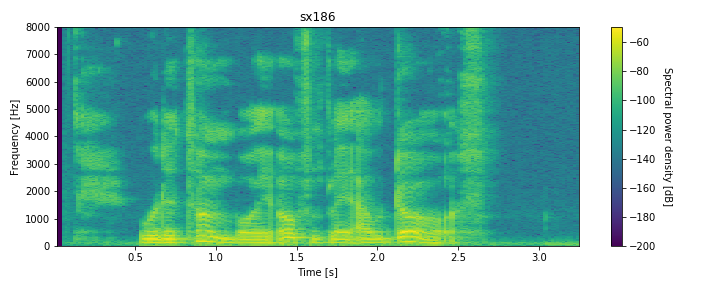
\includegraphics[width=\linewidth]{./sx186_spectogram.png}
	\caption{Would a tomboy often play outdoors?}
\end{figure}


\end{document}